%!TEX root = ../report.tex
%%%%%%%%%%%%%%%%%%%%%%%%%%%%%%%%%%%%%%%%%%%%%%%%%%%%%%%%%%%%%%%%%%%%%%%
%%%%%%%%%%%%%%%%%%%%%%%%%%%%%%%%%%%%%%%%%%%%%%%%%%%%%%%%%%%%%%%%%%%%%%%
%%%%%                                                                 %
%%%%%     <file_name>.tex                                             %
%%%%%                                                                 %
%%%%% Author:      Florian Zaruba                                     %
%%%%% Created:     <date>                                             %
%%%%% Description: <description>                                      %
%%%%%                                                                 %
%%%%%%%%%%%%%%%%%%%%%%%%%%%%%%%%%%%%%%%%%%%%%%%%%%%%%%%%%%%%%%%%%%%%%%%
%%%%%%%%%%%%%%%%%%%%%%%%%%%%%%%%%%%%%%%%%%%%%%%%%%%%%%%%%%%%%%%%%%%%%%%


\chapter{Theory / Algorithms}
% Describe the algorithms you evaluated. The \textit{algorithmic} flow
% of your work should be clear after this chapter. Do not talk much
% about the resulting hardware architecture as this is a different topic
% (next chapter)! If you performed any number precision evaluations put
% them in this chapter as well.

\section{FreeRTOS}

FreeRTOS is a popular, well-supported, open-source real time operating system published under GPL. It is widely used throughout the industry for various projects and it sees itself as the de-facto standard solution for microcontroller and small microprocessors. It underlies strong peer reviewed quality control and provides the developer with well documented sources.

With its highly configurable nature it allows for preemptive scheduling as well as cooperative scheduling. Additionally it offers queues for inter process communication (IPC) and synchronization constructs through critical sections and mutual exclusion (mutex). It can also make use of more advanced hardware features like a memory protection unit (MPU) and different privilege levels.

The hardware dependent code is cleanly separated through a distinct portable layer that abstracts all hardware related features. This makes it easily possible to port application code between two different devices albeit their architectural differences. The operating system (OS) specific implementations like the scheduler and synchronization constructs are entirely written in C and therefore architecture independent. Depending on your resources and requirements it is possible to employ different memory allocations schemes. Several implementations are shipped with freeRTOS itself but you are free to implement your own allocation scheme. The shipped allocation schemes start from simple block based array allocation up to calls to standard (newlib) C library functions \verb+malloc()+ and \verb+free()+.

To my extent this is the first implementation of a RISC-V portable layer. Although the implementation makes use of non (yet) standardized features like interrupts and timers it should be no big problem to adapt it for feature use of the standardized facilities.

\subsection{Purpose of an Operating System}

The purpose of an OS can be manifold. But what unites them all is the purpose to share computational resources between different tasks (programs, processes). Essentially giving the application user the feeling as if the programs are executed in parallel. It therefore distributes the processing time amongst each of the programs. Furthermore it should be possible for the tasks to communicate with each other and to acquire shared resources (for example I/O or a shared variable). This is especially true for the case of freeRTOS.

In freeRTOS scheduling is provided in two different ways. On the one hand it maintains a preemptive scheduler that can preempt the currently running task and give execution time to another task. On the other hand freeRTOS has a cooperative scheduling algorithm as well. This means that the program given control to, essentially runs as long as it returns control back to the OS. There is no way for the OS to interrupt the currently running task by any means. The process of switching between tasks is called context switch. Nevertheless freeRTOS uses the tick interrupt in this setting as well in order to figure out how long the task has been running and to eventually schedule a different task accordingly.

Regardless of the scheduling scheme it is crucial for the OS to be able to track whether a task is ready to run or e.g.: has previously been suspended. It therefore assigns it to different states depending on the reason the task was swapped out beforehand. In freeRTOS a task can be in one of the following four states:

\begin{figure}[htbp]
 \centering
 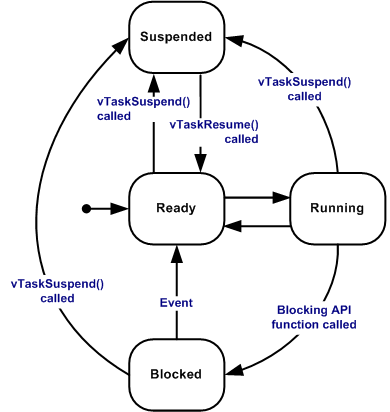
\includegraphics[width=0.6\linewidth]{./figures/tskstate.png}
 \caption{FreeRTOS task state diagram. TODO: list resource}
 \label{fig:task_states}
\end{figure}


\begin{itemize}
    \item Running: When a task is actually utilizing the processor it is said to be in the running state.
    \item Ready: A task is said to be ready if it is not utilizing the core at the moment (it is not in the running state) but is ready to run as soon as the OS decides to switch it in.
    \item Blocked: A process is blocked if it currently waiting for a temporal (e.g.: a timed delay) or an external event (e.g.: release of a shared resource).
    \item Suspended: A task is suspended if it has been told so through an explicit function call to \verb+vTaskSuspend()+.
\end{itemize}

The whole state diagram is depicted in figure~\ref{fig:task_states}. When a task gets switched in the scheduling algorithm has to decided which new task is given processor time. There are different approaches to that. For example a round robin scheduler assigns fixed time slots to every process and the different tasks are therefore provided with equal computation time. FreeRTOS pursues a slightly different approach. At the creation of each task the programmer can assign a priority to the task he is creating. Based on the priority freeRTOS schedules the next task accordingly, beginning with the highest priority task either in the ready or running state. Least precedence is given to lower priority tasks. The idle task has priority zero. If two tasks share the same priority freeRTOS schedules them in a round robin fashion.

\begin{figure}[htbp]
 \centering
 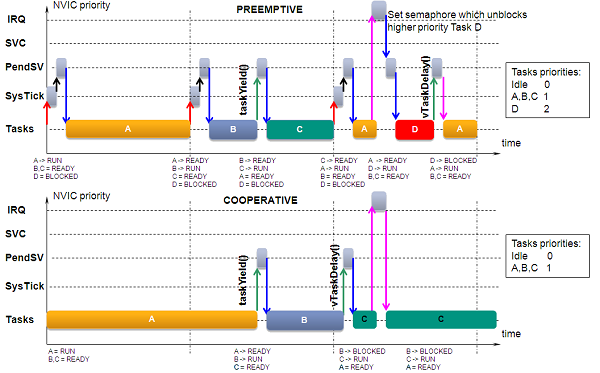
\includegraphics[width=\linewidth]{./figures/preemptive_cooperative.png}
 %https://www.rapitasystems.com/blog/cooperative-and-preemptive-scheduling-algorithms
 \caption{Preemptive and cooperative context switch}
 \label{fig:context_switch}
\end{figure}


In the preemptive case the OS needs a way to preempt a currently running task. It does this by registering a interrupt service routine (ISR) triggered by a timer that is configured by the OS according to the users specification. The interrupt triggers an asynchronous change in the control flow and directs control back to the OS that then decides whether the current task shall be switch out or not. Figure~\ref{fig:context_switch} depicted the difference between a preemptive and cooperative context switch.

\subsection{Directory structure}

Since freeRTOS aims high portability, the directory structure directly reflects this property. Everything that is architectural specific resides in the \verb+portable+ folder. This begins with basic configuration macros and continues with implementation of the actual context switch in \verb+port.c+.

\begin{minipage}{\linewidth}
\begin{flushleft}
\dirtree{%
.1 /.
  .2 main.c \DTcomment{Entry point of user program}.
  .2 FreeRTOSConfig.h \DTcomment{User defined and application specific freeRTOS configuration}.
  .2 update-ips.py \DTcomment{This script reads the ip\_list.txt and pulls all ips from the GIT server}.
  .2 include \DTcomment{Folder containing scripts used by continuous integration}.
  .2 portable \DTcomment{Contains the actual source files of your report.}.
    .3 GCC \DTcomment{Portable layer specific to GCC}.
        .3 RI5CY \DTcomment{Portable layer specific to the microcontroller's architecture}.
            .4 portmacro.h \DTcomment{architecture related configuration file}.
            .4 port.c \DTcomment{Actual portable layer implementation}.
    .3 MemMang \DTcomment{Memory management schemes.}.
  .2 event\_groups.c \DTcomment{freeRTOS eventing scheme.}.
  .2 list.c \DTcomment{List implementation - Task utility}.
  .2 tasks.c \DTcomment{Task implementation.}.
  .2 timers.c \DTcomment{Software timers.}.
}
\end{flushleft}
\end{minipage}
\subsection{Portable layer}

The portable layers purpose is to abstract all device specific information to the OS. In particular this means implementation of the actual context switch, interrupt service routines (ISRs) that trigger the context switch and stack initialization for task creation. All device specific codes resides here.

\subsection{Context Switch}

\begin{figure}[t]
 \centering
 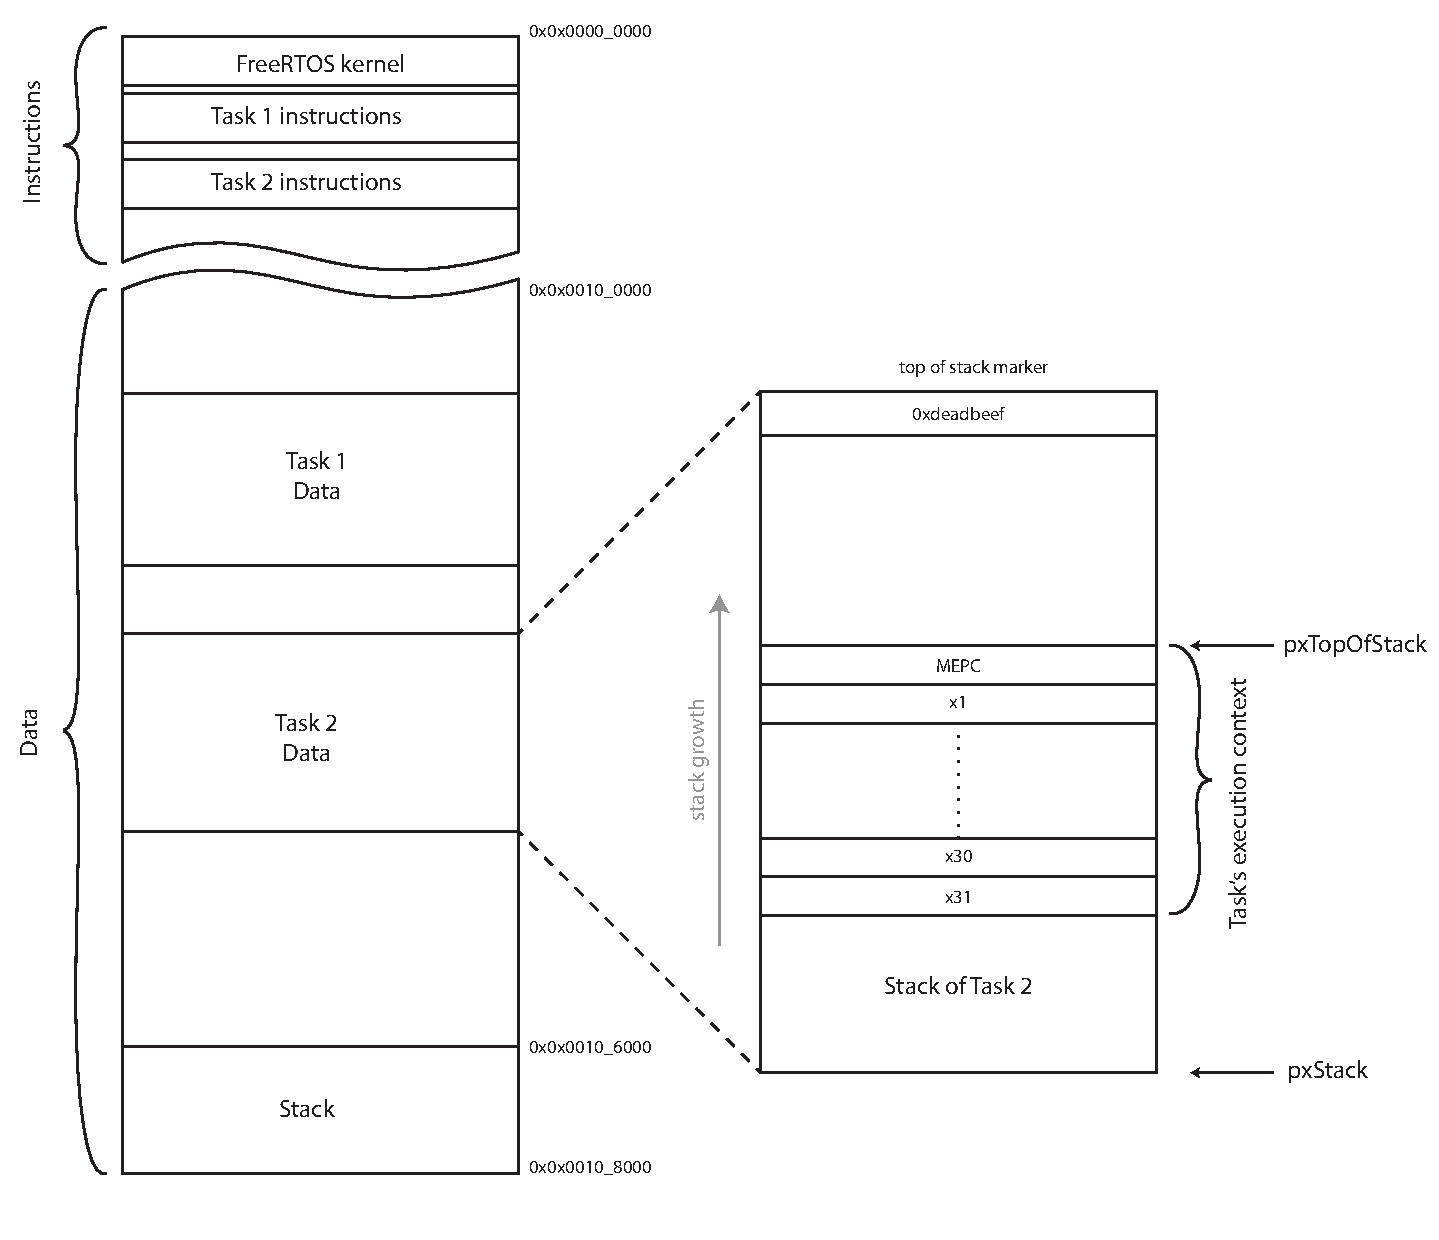
\includegraphics[width=\linewidth]{./figures/freertos_memorymap}
 %https://www.rapitasystems.com/blog/cooperative-and-preemptive-scheduling-algorithms
 \caption{FreeRTOS memory management and stack content of a switched out task (Task 2)}
 \label{fig:memory_management}
\end{figure}

Context switches can occur in two different settings depending on the scheduling algorithm in use. According to that, there are differences in the program control flow. Nevertheless the main idea of the context switch stays the same.

Each task in freeRTOS manages its own stack (figure~\ref{fig:memory_management}). The task's memory region is allocated when the tasks gets registered for the first time and reside entirely in the heap regardless of the global linker settings. In order for FreeRTOS to manage the task's memories it stores task related information in its own task structure called Task Control Block (TCB). The TCB has essentially the following structure:

\begin{figure}[t]
 \centering
 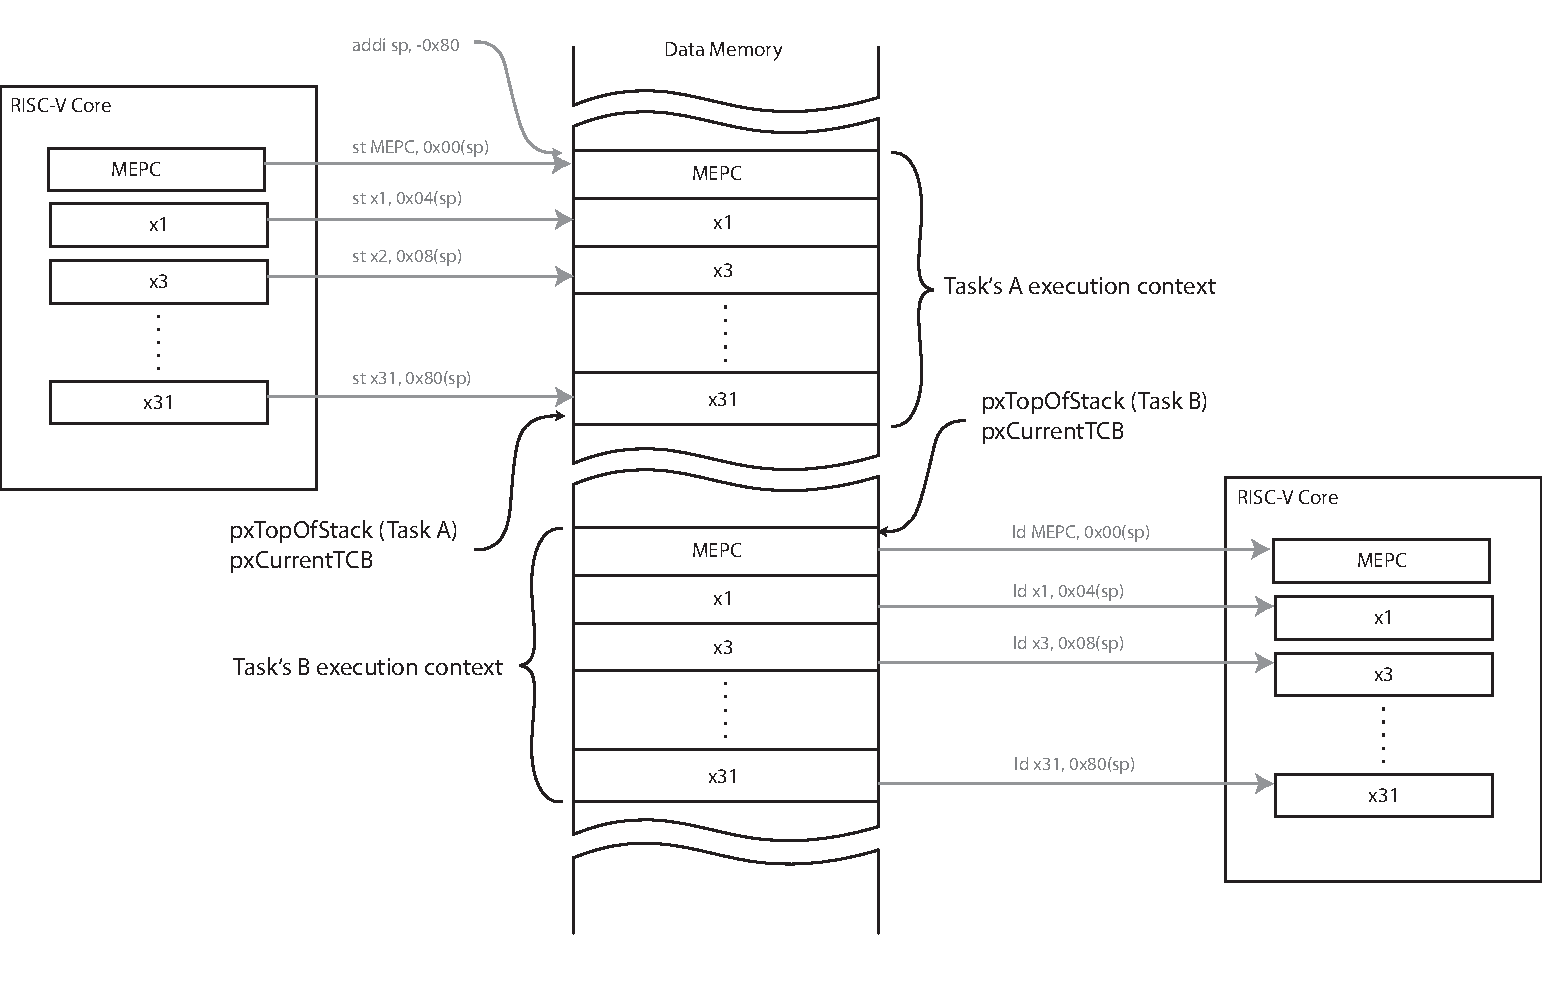
\includegraphics[width=\linewidth]{./figures/freertos_context_switch}
 %https://www.rapitasystems.com/blog/cooperative-and-preemptive-scheduling-algorithms
 \caption{FreeRTOS context switch}
 \label{fig:context_switch}
\end{figure}

%memory layout
\begin{minipage}{\linewidth}
\begin{lstlisting}[language=C,emph={xListItem,portSTACK_TYPE}]
typedef struct tskTaskControlBlock
{
  volatile portSTACK_TYPE *pxTopOfStack;
  xListItem    xGenericListItem;
  xListItem    xEventListItem;
  unsigned portBASE_TYPE uxPriority;
  portSTACK_TYPE *pxStack;
  ...
} tskTCB;
\end{lstlisting}
\end{minipage}


The \verb+pxTopOfStack+ variable points to the last element put on the stack of the task and must be the first element of the TCB structure. \verb+pxStack+ on the contrary points to the stack's base address.

If a task is switched out its current state is going to be saved into memory. For the RISC-V RV32I this implies at least all general purpose registers and the MEPC register that has the program counter stored from which the interrupt service unit may return to. It does so by calling the \verb+portSAVE_CONTEXT()+ macro defined in \verb+port.c+. This macro allocates some space on the stack and stores every register in a predefined order, starting with the MEPC. Finally it updates the \verb+pxCurrenTCB+ pointer that points to the TCB of the task switch out and updates the stack pointer. The stack pointer is therefore saved implicitly in the TCB.

The OS then figures out which task that is going to run next (based on the principles mentioned beforehand) and afterwards calls the \verb+portRESTORE_CONTEXT()+ macro. This essentially performs the same function as the save routine but in reverse order, e.g. it loads the stack pointer of the task that is going to be switched in from the pxCurrentTCB and restores all registers from memory in the same order as they have been saved.

% picture

For the cooperative case this happens within a normal function call, e.g.: a task decides that it may wants to yield and therefore gives a call to \verb+vPortYield()+. The scheduler saves the current context and restores it after it has figured out which task is going to be switched in. It is crucial that the save and restore sequence does not get interrupted therefore interrupts are disabled throughout the whole process.

For the preemptive case this happens within an ISR. The only difference to the cooperative case is that the return from the interrupt (ERET) will use the MEPC register to find out where the current task has been interrupted from.

\subsubsection{Context Switch Overhead}

It is crucial for the property as a real time operating system to know exactly how long (in terms of processing time) certain sequences of code need. While this is often very difficult to state for more complex systems this is quite feasible in the context of a single core microcontroller and especially for \pulpino. For the current implementation of freeRTOS I can give this exact cycle time break-down:

\begin{enumerate}
  \item 43 cycles for storing of all registers
  \item 64 cycles for scheduling the next task.
  \item 43 cycles for the restore sequence of all registers
  \item 68 cycles overhead for the interrupt call and all subsequent function calls and returns. Interrupt and function calls need a certain amount of time imposed by the compiler to obey the callee/caller convention (e.g. certain registers need to be saved by the callee and some by the caller of a function).
\end{enumerate}

This makes a total of 218 cycles for the overall context switch e.g. from the time of one task becoming suspended to the time another tasks starts executing.

\subsection{Stack initialization}

The purpose of the stack initialization is to setup a task structure in the data RAM to look like it has been already running and was only switched out by the scheduler. To this point the OS has already allocated some space on the stack. What remains for the initialization to do is to store the start address of the task on the same place we would have stored the return address (register x1) and the MEPC if the task has been switched out. It therefore can simply restore the context of the task albeit it has never been running before.

Remaining functionality that is architecture depended is the configuration of the timer interrupt and a call to return to directly jump to the tasks code. We have to manually call the \verb+ret+ directive since we do not want to return to the function that has called \verb+xPortStartScheduler+ but to the program.

